\documentclass[10pt,a4paper]{article}

\usepackage[a4paper,margin=0.9in]{geometry}
\usepackage[T1]{fontenc}
\usepackage[utf8]{inputenc}
\usepackage{lmodern}
\usepackage{microtype}
\usepackage{setspace}
\usepackage{graphicx}
\usepackage{xcolor}
\usepackage{booktabs}
\usepackage{tabularx}
\usepackage{array}
\usepackage{float}
\usepackage{tikz}
\usetikzlibrary{arrows.meta,positioning,shapes.geometric,calc}
\usepackage[hidelinks]{hyperref}
\usepackage{caption}
\usepackage{titlesec}

\setlength{\parindent}{0pt}
\setlength{\parskip}{0.35em}
\linespread{1.04}
\captionsetup{font=small,labelfont=bf}
\titleformat{\section}{\Large\bfseries}{\thesection.}{0.5em}{}
\titleformat{\subsection}{\large\bfseries}{\thesubsection}{0.5em}{}

\newcommand{\placeholderbox}[2]{%
    \fbox{%
        \parbox[c][#2][c]{0.82\linewidth}{%
            \centering #1
        }%
    }%
}

\begin{document}

% SECTION 1 --- Cover Page
\begin{titlepage}
\centering
\vspace*{1.2cm}

{\Huge\bfseries Reliable Underwater Optical Communication Using Smartphones\par}
\vspace{0.6cm}
{\Large\itshape Mentored by Prof.~Arnab Paul\par}
\vspace{1.0cm}

\renewcommand{\arraystretch}{1.35}
\begin{tabular}{>{\bfseries}l l}
Vishrut Ramraj & 2023A7PS0352G \\
Ragav Krishna Ramesh & 2023A7PS0415G \\
\end{tabular}

\vspace{1.3cm}
\IfFileExists{logo.png}{%
    \includegraphics[width=0.26\textwidth]{logo.png}
}{%
    \placeholderbox{BITS Pilani Logo Placeholder\\Place \texttt{logo.png} in project root.}{5.1cm}
}

\vfill
{\large Submitted on March 1, 2026\par}
\end{titlepage}

% Table of contents page
\tableofcontents
\newpage

% Start section numbering from 2 because cover page is Section 1.
\setcounter{section}{1}

% SECTION 2 --- Abstract
\section{Abstract}
We built an underwater phone-to-phone optical communication system using only flashlight TX and camera RX. The receiver uses ROI grid analysis, rolling histograms, Otsu confidence, and ON-duration decoding at 20 FPS. The protocol layer includes constants, packet framing, CRC-8, and an FSM for session flow. In the final deliverable, reliable manual packet transfer works for fixed transmitter/receiver positions with 5-character packets.

% SECTION 3 --- Problem Statement
\section{Problem Statement}
The goal is reliable underwater communication between two smartphones with no external hardware. The system is constrained by camera frame rate, torch latency, sensor noise, ambient-light variation, and device motion.

Underwater scattering and reflections reduce ON/OFF contrast, and camera auto-exposure can suppress flash differences in a few frames. Therefore, we run a fixed 20 FPS camera path with manual exposure and decode transitions instead of sustained brightness.

The design target is low BER and stable packet decode success under these constraints, using timing margins, CRC checks, and retransmission logic.

% SECTION 4 --- High-Level System Architecture
\section{High-Level System Architecture}
This report includes both implemented components and explored approaches from the hackathon. Sections 2--11 cover the full system and attempted protocol path; Section 12 (\textit{What Actually Works? / Final Deliverables}) states what is currently working reliably.

\subsection{Architecture Diagram}
\begin{figure}[H]
\centering
\resizebox{0.98\linewidth}{!}{%
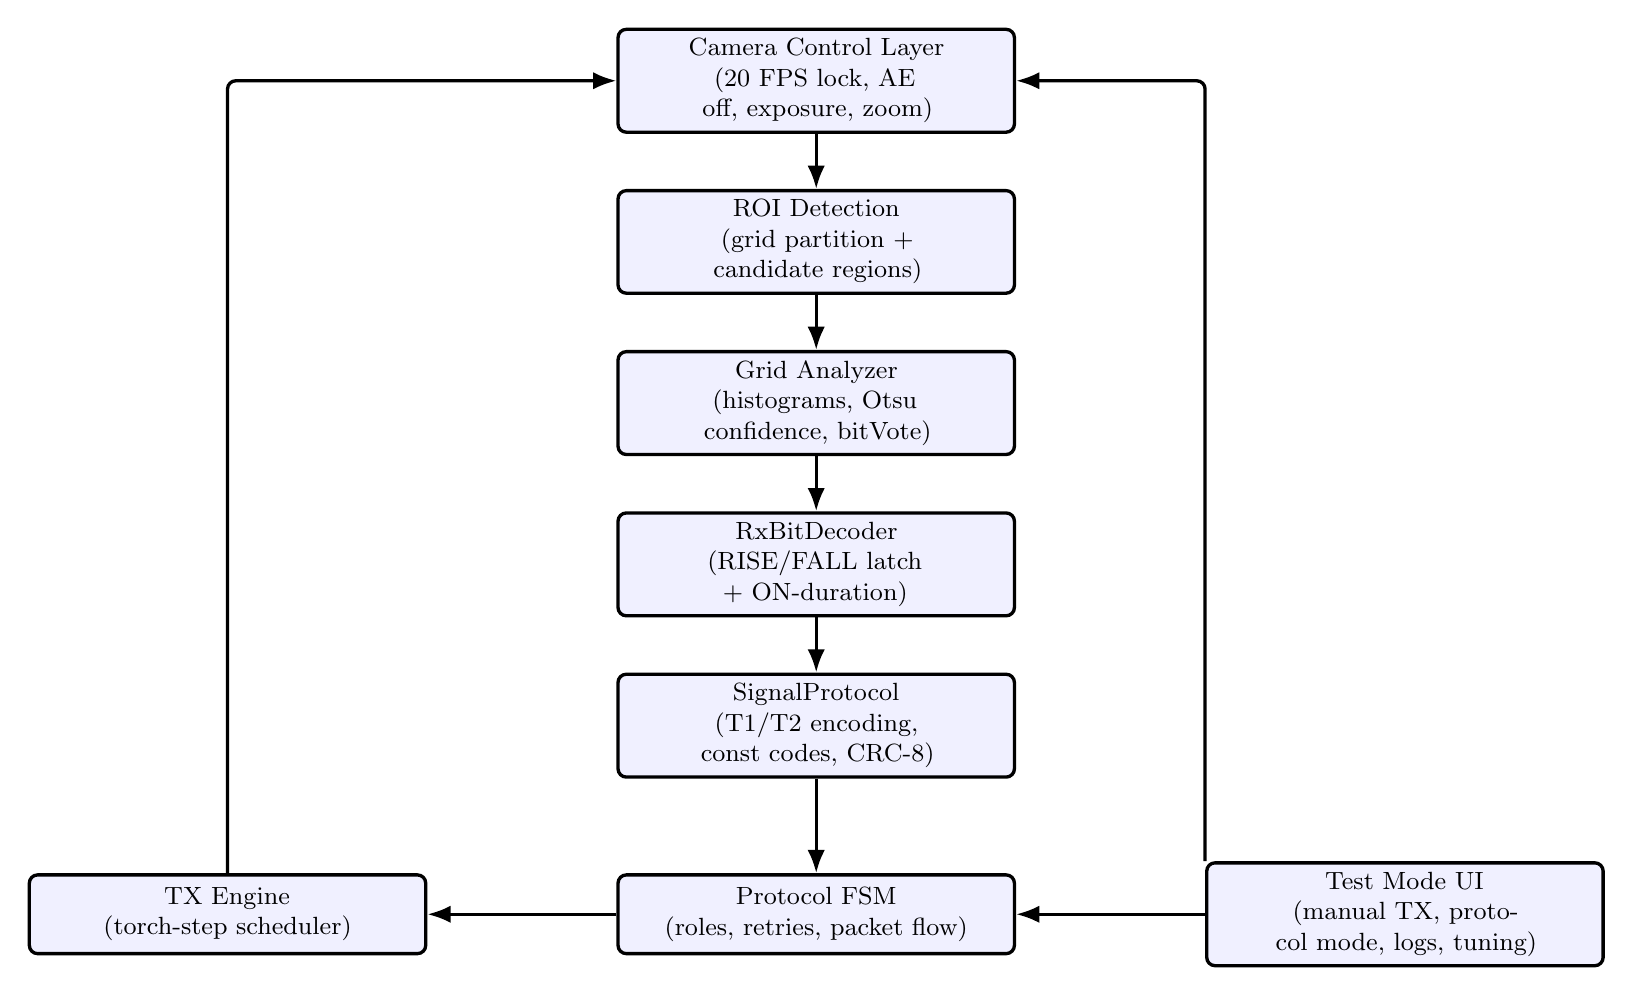
\begin{tikzpicture}[
    module/.style={rectangle, rounded corners=3pt, draw=black, very thick, fill=blue!6, text width=4.8cm, minimum height=1.0cm, align=center, font=\small},
    arrow/.style={-Latex, very thick, rounded corners=3pt}
]
\node[module] (cam) {Camera Control Layer\\(20 FPS lock, AE off, exposure, zoom)};
\node[module, below=7mm of cam] (roi) {ROI Detection\\(grid partition + candidate regions)};
\node[module, below=7mm of roi] (grid) {Grid Analyzer\\(histograms, Otsu confidence, bitVote)};
\node[module, below=7mm of grid] (rx) {RxBitDecoder\\(RISE/FALL latch + ON-duration)};
\node[module, below=7mm of rx] (sig) {SignalProtocol\\(T1/T2 encoding, const codes, CRC-8)};
\node[module, below=12mm of sig] (fsm) {Protocol FSM\\(roles, retries, packet flow)};
\node[module, left=24mm of fsm] (tx) {TX Engine\\(torch-step scheduler)};
\node[module, right=24mm of fsm] (ui) {Test Mode UI\\(manual TX, protocol mode, logs, tuning)};

\draw[arrow] (cam) -- (roi);
\draw[arrow] (roi) -- (grid);
\draw[arrow] (grid) -- (rx);
\draw[arrow] (rx) -- (sig);
\draw[arrow] (sig) -- (fsm);
\draw[arrow] (fsm) -- (tx);
\draw[arrow] (tx.north) |- (cam.west);
\draw[arrow] (ui.west) -- (fsm.east);
\draw[arrow] (ui.north west) |- (cam.east);
\end{tikzpicture}%
}
\caption{High-level module flow for the underwater communication stack.}
\end{figure}

\subsection{High-Level Design Explanation}
The pipeline is layered: camera control stabilizes acquisition, ROI/grid modules estimate signal strength, the bit decoder extracts T1/T2 bits, and protocol modules map bits to constants and packet operations. This separation allows quick tuning of physical parameters (grid, threshold, window, zoom) without changing protocol logic.

The UI supports up to 80 input characters for testing. The current mapping uses lowercase letters plus basic punctuation and space, and the encoding layer can be extended later.

% SECTION 5 --- ROI Detection Algorithm
\section{ROI Detection Algorithm}
At 20 FPS (480p), each frame is split into grids. Each grid keeps a short brightness history; high-confidence connected grids form the active cluster used for decoding.

Per-grid histograms are thresholded with Otsu. Bimodal histograms produce high confidence, while unimodal regions drop toward zero confidence. This suppresses static bright areas and background glare.

The receiver depends on transitions, not sustained ON/OFF states. Sustained states collapse histograms into one mode, reducing confidence and weakening bit votes. Rolling-window mode with \(N=3\) gives sharp transition spikes and stable adapted zero regions, which makes edge timing reliable.

\begin{table}[H]
\centering
\caption{Main ROI and decoder hyperparameters used during tuning.}
\begin{tabularx}{\linewidth}{>{\bfseries}l c X}
\toprule
Parameter & Typical value & Practical role \\
\midrule
Alpha decay (\texttt{alpha}) & 0.05 & Histogram adaptation speed in alpha-decay mode. Lower values are more stable; higher values react faster. \\
Confidence threshold & 0.15 & Minimum Otsu confidence for a grid to be treated as active. \\
Vote threshold (\texttt{VOTE\_THRESH}) & 0.25 & Threshold for bright/dark edge latching in rolling-window mode. \\
Grid size & 8 px & Smaller grids improve spatial precision; larger grids average noise better. \\
Window size (\(N\)) & 3 frames & Controls temporal smoothing in rolling-window mode. \\
\bottomrule
\end{tabularx}
\end{table}

Tuning is environment-dependent: low light may need larger grids/lower confidence threshold, while flickering backgrounds may need stricter thresholds. Zoom (1x, 2x, 4x) is a practical SNR control; higher zoom usually helps at longer distances.

% SECTION 6 --- Type 1 and Type 2 Binary Encodings
\section{Type 1 and Type 2 Binary Encodings}

\subsection{Type 1 (T1) Bit Encoding}
Type 1 encodes packet bits with a fixed 600 ms window using ON-duration plus OFF-duration.

\begin{table}[H]
\centering
\caption{Type 1 timings.}
\begin{tabular}{lcc}
\toprule
Bit value & ON duration & OFF duration \\
\midrule
0 & 200 ms & 400 ms \\
1 & 400 ms & 200 ms \\
\bottomrule
\end{tabular}
\end{table}

\begin{figure}[H]
\centering
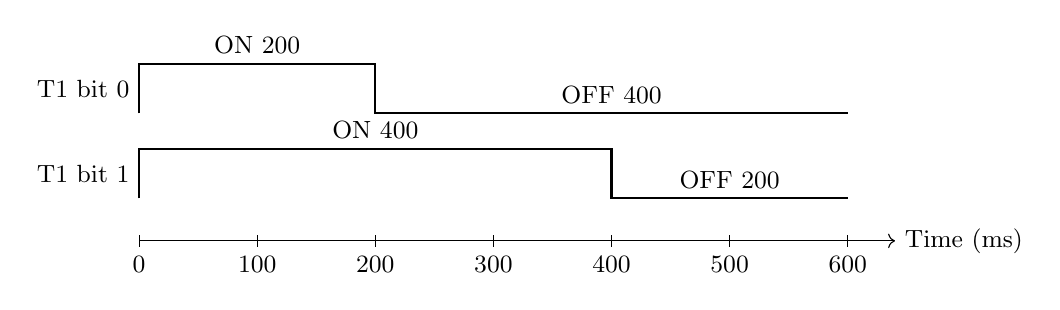
\begin{tikzpicture}[x=0.015cm,y=0.9cm,font=\small]
\draw[->] (0,0) -- (640,0) node[right]{Time (ms)};
\foreach \x in {0,100,200,300,400,500,600} {
    \draw (\x,0.08) -- (\x,-0.08);
    \node[below] at (\x,-0.08) {\x};
}

\draw[thick] (0,1.8) -- (0,2.5) -- (200,2.5) -- (200,1.8) -- (600,1.8);
\node[left] at (0,2.15) {T1 bit 0};
\node[above] at (100,2.5) {ON 200};
\node[above] at (400,1.8) {OFF 400};

\draw[thick] (0,0.6) -- (0,1.3) -- (400,1.3) -- (400,0.6) -- (600,0.6);
\node[left] at (0,0.95) {T1 bit 1};
\node[above] at (200,1.3) {ON 400};
\node[above] at (500,0.6) {OFF 200};
\end{tikzpicture}
\caption{Type 1 ON-duration timing diagram (600 ms per bit).}
\end{figure}

At 20 FPS (50 ms/frame), 200 ms and 400 ms ON clusters remain separable under frame jitter.

\subsection{Type 2 (T2) Bit Encoding}
Type 2 is used for constant/control symbols with a 1800 ms bit window.

\begin{table}[H]
\centering
\caption{Type 2 timings.}
\begin{tabular}{lcc}
\toprule
Bit value & ON duration & OFF duration \\
\midrule
0 & 600 ms & 1200 ms \\
1 & 1200 ms & 600 ms \\
\bottomrule
\end{tabular}
\end{table}

\begin{figure}[H]
\centering
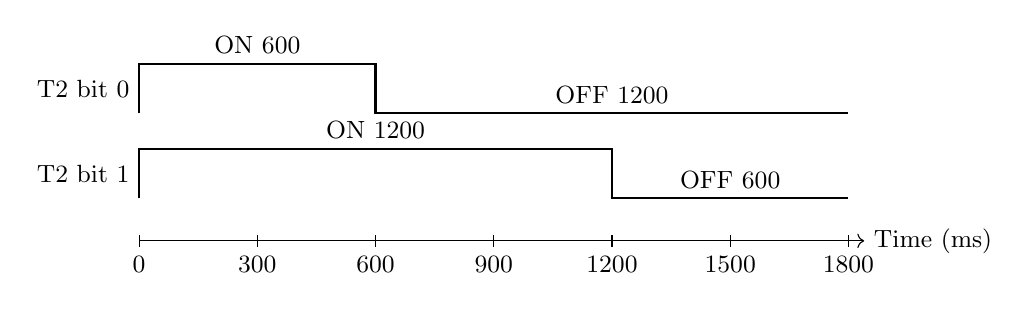
\begin{tikzpicture}[x=0.005cm,y=0.9cm,font=\small]
\draw[->] (0,0) -- (1840,0) node[right]{Time (ms)};
\foreach \x in {0,300,600,900,1200,1500,1800} {
    \draw (\x,0.08) -- (\x,-0.08);
    \node[below] at (\x,-0.08) {\x};
}

\draw[thick] (0,1.8) -- (0,2.5) -- (600,2.5) -- (600,1.8) -- (1800,1.8);
\node[left] at (0,2.15) {T2 bit 0};
\node[above] at (300,2.5) {ON 600};
\node[above] at (1200,1.8) {OFF 1200};

\draw[thick] (0,0.6) -- (0,1.3) -- (1200,1.3) -- (1200,0.6) -- (1800,0.6);
\node[left] at (0,0.95) {T2 bit 1};
\node[above] at (600,1.3) {ON 1200};
\node[above] at (1500,0.6) {OFF 600};
\end{tikzpicture}
\caption{Type 2 ON-duration timing diagram (1800 ms per bit).}
\end{figure}

\subsection{Why ON-Duration Encoding and 100 ms Margins}
ON-duration encoding is robust because decoding uses RISE/FALL timing instead of absolute brightness. The 100 ms gaps between timing classes (two frames at 20 FPS) prevent class overlap in normal jitter.

% SECTION 7 --- Character Encoding (5-bit)
\section{Character Encoding (5-bit)}
Packet payload uses fixed 5-bit symbols for deterministic timing and simple decoding.

\begin{table}[H]
\centering
\caption{5-bit character mapping used in the current system.}
\begin{tabular}{lll}
\toprule
5-bit code / index & Character set & Note \\
\midrule
00000 to 11001 (0 to 25) & a to z & Lowercase alphabets \\
11010 (26) & , & Comma \\
11011 (27) & . & Period \\
11100 (28) & ! & Exclamation \\
11101 (29) & ? & Question mark \\
11110 (30) & [space] & Space character \\
11111 (31) & PAD & Null padding marker \\
\bottomrule
\end{tabular}
\end{table}

Fixed width keeps packet timing constant and receiver logic simple.

\subsection{Exploration: Custom Balanced Huffman Encoding (Discarded Idea)}
We explored balanced Huffman coding to reduce average bits per character. It reduced average length in theory, but variable-length symbols introduced variable timing and harder boundary detection. We therefore kept fixed 5-bit symbols.

\begin{figure}[H]
\centering
\IfFileExists{balanced_huffman.png}{%
    \includegraphics[width=0.88\linewidth]{balanced_huffman.png}
}{%
    \placeholderbox{Balanced Huffman Exploration Placeholder\\Place \texttt{balanced\_huffman.png} in project root.}{5.0cm}
}
\caption{Exploratory balanced Huffman design (not used in final protocol).}
\end{figure}

% SECTION 8 --- Packet Structure
\section{Packet Structure}
Each packet carries 5 characters: 25 data bits + 8 CRC bits = 33 bits total.

\begin{figure}[H]
\centering
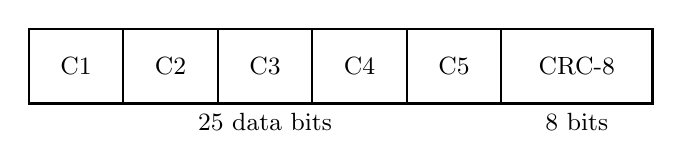
\begin{tikzpicture}[x=0.24cm,y=0.95cm,font=\small]
\draw[thick] (0,0) rectangle (33,1);
\draw[thick] (5,0) -- (5,1);
\draw[thick] (10,0) -- (10,1);
\draw[thick] (15,0) -- (15,1);
\draw[thick] (20,0) -- (20,1);
\draw[thick] (25,0) -- (25,1);
\node at (2.5,0.5) {C1};
\node at (7.5,0.5) {C2};
\node at (12.5,0.5) {C3};
\node at (17.5,0.5) {C4};
\node at (22.5,0.5) {C5};
\node at (29,0.5) {CRC-8};
\node[below] at (12.5,0) {25 data bits};
\node[below] at (29,0) {8 bits};
\end{tikzpicture}
\caption{Packet bit layout: 5 characters + CRC-8.}
\end{figure}

All packet bits use Type 1 timing, so one packet takes \(33 \times 600\) ms \(= 19.8\) seconds. PAD fills short inputs to 5 characters.

Example payload: \texttt{"hi, ?"}.
\begin{center}
\texttt{h = 00111,\ i = 01000,\ , = 11010,\ [space] = 11110,\ ? = 11101}
\end{center}
These data bits are followed by CRC-8 (polynomial \(0x07\), CRC8-CCITT) before transmission.

\begin{table}[H]
\centering
\caption{Example CRC mismatch behavior for one-bit corruption.}
\begin{tabular}{ll}
\toprule
Transmitted packet & Data bits \(D\) + CRC \(C\) \\
Received packet & Data bits \(D'\) (one bit flipped) + same CRC \(C\) \\
Receiver check & Recomputed CRC \(C' \neq C\), packet rejected and retransmitted \\
\bottomrule
\end{tabular}
\end{table}

% SECTION 9 --- Signals / Constant Sequences
\section{Signals / Constant Sequences}
Control signals use 3-bit Type 2 encoding for robust constant detection.

\begin{table}[H]
\centering
\caption{Constant signal definitions.}
\begin{tabular}{lccc}
\toprule
Signal & 3-bit value & Encoding type & Duration \\
\midrule
C1 & 000 & T2 (3 bits) & 5400 ms \\
C2 & 001 & T2 (3 bits) & 5400 ms \\
C3 & 010 & T2 (3 bits) & 5400 ms \\
R  & 011 & T2 (3 bits) & 5400 ms \\
S  & 100 & T2 (3 bits) & 5400 ms \\
E  & 101 & T2 (3 bits) & 5400 ms \\
Q  & 110 & T2 (3 bits) & 5400 ms \\
\bottomrule
\end{tabular}
\end{table}

\subsection*{Q:no Special Case}
\texttt{Q:no} is a mixed-format frame:
\begin{itemize}
\item \texttt{Q} is transmitted as 3 T2 bits (\(5400\) ms).
\item The packet number \texttt{no} is transmitted as 4 T1 bits (\(2400\) ms).
\end{itemize}
Total duration is \(5400 + 2400 = 7800\) ms.

Example for requesting packet 3:
\begin{center}
\texttt{Q (110 in T2)} + \texttt{0011 (packet no in T1)}
\end{center}
T2 is used for a robust constant prefix, while T1 keeps packet-number transmission short.

% SECTION 10 --- Protocol FSM
\section{Protocol FSM}

\begin{figure}[H]
\centering
\resizebox{0.98\linewidth}{!}{%
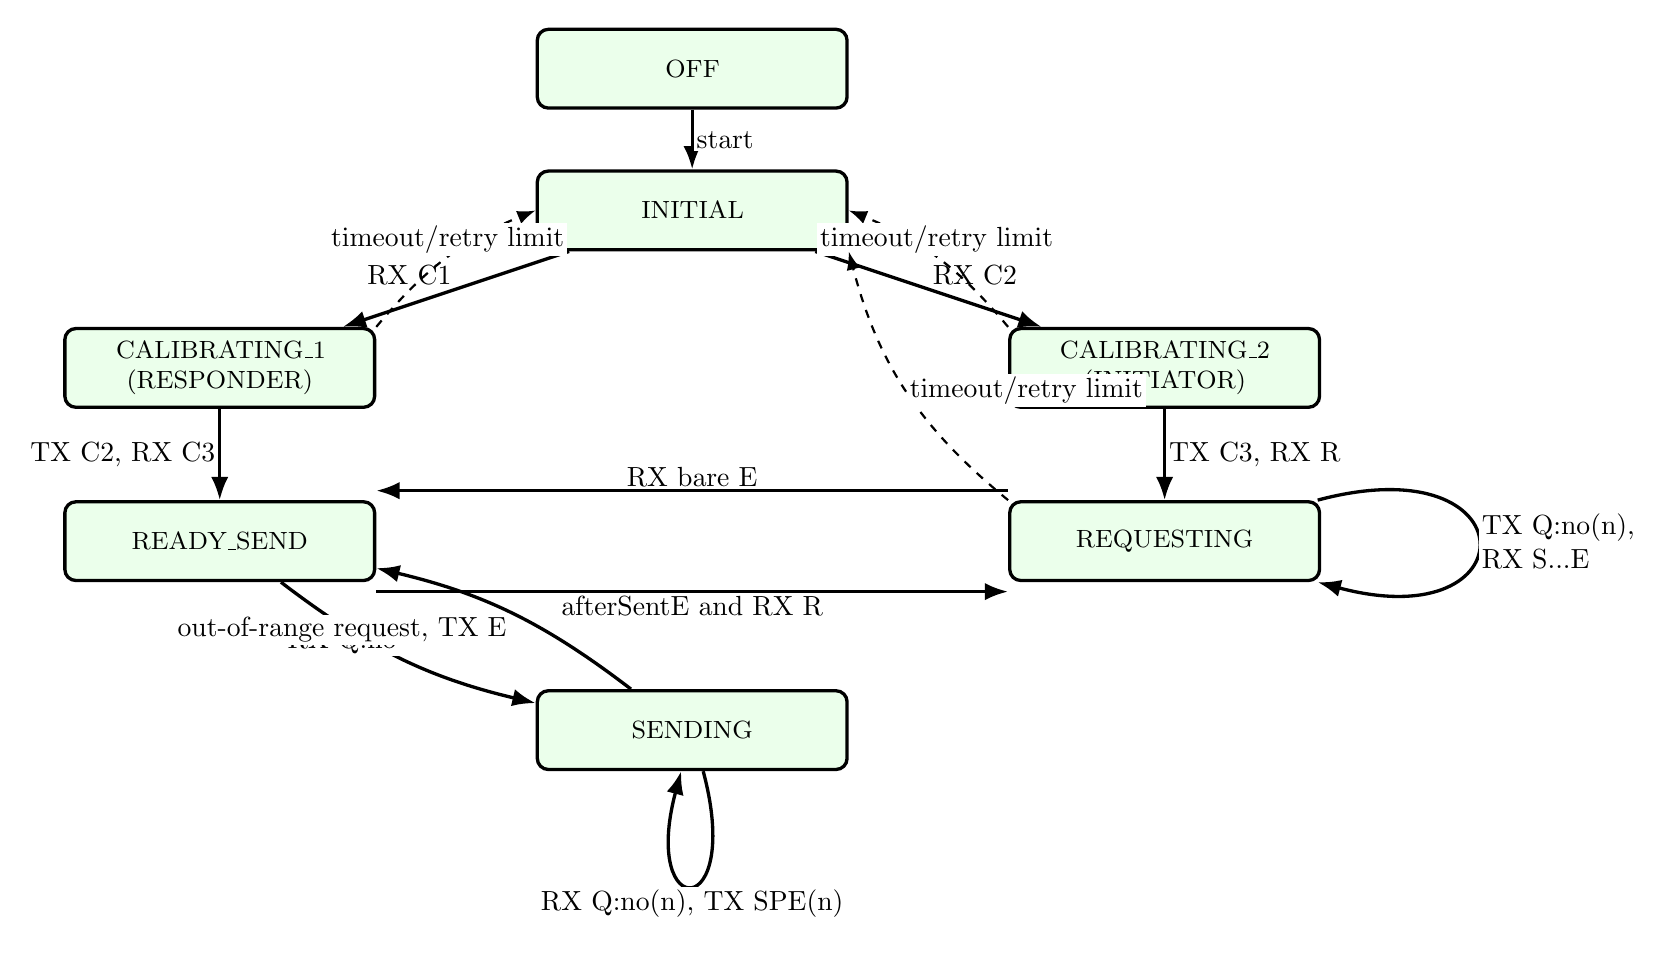
\begin{tikzpicture}[
    state/.style={rectangle, rounded corners=4pt, draw=black, very thick, fill=green!8, text width=3.7cm, minimum height=1.0cm, align=center, font=\small},
    arr/.style={-Latex, very thick},
    darr/.style={-Latex, thick, dashed}
]
\node[state] (off) at (0,7.0) {OFF};
\node[state] (initial) at (0,5.2) {INITIAL};
\node[state] (c1) at (-6.0,3.2) {CALIBRATING\_1\\(RESPONDER)};
\node[state] (c2) at (6.0,3.2) {CALIBRATING\_2\\(INITIATOR)};
\node[state] (ready) at (-6.0,1.0) {READY\_SEND};
\node[state] (req) at (6.0,1.0) {REQUESTING};
\node[state] (send) at (0,-1.4) {SENDING};

\draw[arr] (off) -- node[right, fill=white, inner sep=1pt]{start} (initial);
\draw[arr] (initial) -- node[above left, fill=white, inner sep=1pt]{RX C1} (c1);
\draw[arr] (initial) -- node[above right, fill=white, inner sep=1pt]{RX C2} (c2);
\draw[arr] (c1) -- node[left, fill=white, inner sep=1pt]{TX C2, RX C3} (ready);
\draw[arr] (c2) -- node[right, fill=white, inner sep=1pt]{TX C3, RX R} (req);

\draw[arr] (ready) to[bend right=12] node[above left, fill=white, inner sep=1pt]{RX Q:no} (send);
\draw[arr] (send) to[bend right=12] node[below left, fill=white, inner sep=1pt]{out-of-range request, TX E} (ready);

\draw[arr] (req) edge[loop right, min distance=28mm] node[right, align=left, fill=white, inner sep=1pt]{TX Q:no(n),\\RX S...E} (req);
\draw[arr] (send) edge[loop below, min distance=20mm] node[below, align=center, fill=white, inner sep=1pt]{RX Q:no(n), TX SPE(n)} (send);

\draw[arr] ($(req.north west)+(0,0.12)$) -- node[above, fill=white, inner sep=1pt]{RX bare E} ($(ready.north east)+(0,0.12)$);
\draw[arr] ($(ready.south east)+(0,-0.12)$) -- node[below, fill=white, inner sep=1pt]{afterSentE and RX R} ($(req.south west)+(0,-0.12)$);

\draw[darr] (c1.north east) to[bend left=14] node[above, fill=white, inner sep=1pt]{timeout/retry limit} (initial.west);
\draw[darr] (c2.north west) to[bend right=14] node[above, fill=white, inner sep=1pt]{timeout/retry limit} (initial.east);
\draw[darr] (req.north west) to[bend left=18] node[right, fill=white, inner sep=1pt]{timeout/retry limit} (initial.south east);
\end{tikzpicture}%
}
\caption{Protocol finite state machine for session setup and packet exchange.}
\end{figure}

The FSM separates roles: responder path (\texttt{C1} detected) reaches \texttt{READY\_SEND}, and initiator path (\texttt{C2} detected) reaches \texttt{REQUESTING}. This prevents simultaneous data transmission.

In \texttt{REQUESTING}, nodes send \texttt{Q:no}; in \texttt{SENDING}, nodes answer with \texttt{SPE} or bare \texttt{E}. \texttt{RESPONSE\_DELAY\_MS} (3000 ms) is essential to avoid TX/RX overlap.

% SECTION 11 --- Test Mode UI
\section{Test Mode UI}

\begin{figure}[H]
\centering
\IfFileExists{test_mode_ui.png}{%
    \includegraphics[width=0.95\linewidth]{test_mode_ui.png}
}{%
    \placeholderbox{Test Mode UI Placeholder\\Place \texttt{test\_mode\_ui.png} in project root.}{6.2cm}
}
\caption{Test mode interface used during development and evaluation.}
\end{figure}

The test UI supports manual signals, packet transmission, and full protocol mode in one screen.

\begin{table}[H]
\centering
\caption{UI blocks and their debugging purpose.}
\begin{tabularx}{\linewidth}{>{\bfseries}l X}
\toprule
UI feature & Use in debugging and evaluation \\
\midrule
Manual signal transmit & Sends constants (\texttt{C1/C2/C3/R/S/E/Q}) to validate timing classes and edge detection. \\
Packet transmit & Sends packet-form payloads to test 5-bit mapping, CRC behavior, and packet duration. \\
Full protocol controls & Runs the FSM flow end-to-end and validates retries, role changes, and completion handling. \\
Sliding window / mode inputs & Switches histogram mode and window length to compare transition stability. \\
Event log and signal log & Gives a timestamped trace for decoded symbols, state changes, and timeout events. \\
Alpha / threshold inputs & Tunes confidence and edge trigger behavior under different lighting conditions. \\
Grid and zoom controls & Adjusts spatial sampling and SNR in real time (1x, 2x, 4x). \\
\bottomrule
\end{tabularx}
\end{table}

It is the main debugging surface for reproducible timing and state inspection.

% SECTION 12 --- What Actually Works? / Final Deliverables
\section{What Actually Works? / Final Deliverables}
The report includes all protocol work attempted during the hackathon, but the full automated protocol loop was not fully stabilized within the timeline.

What works reliably now is packet TX/RX with end-to-end decoding between fixed transmitter and receiver devices. We can transmit up to 80 characters by splitting the message into packets of 5 characters each and decoding all packets at the receiver.

This behavior is consistent with the current \texttt{SignalProtocol} implementation:
\begin{itemize}
\item \texttt{MAX\_MESSAGE\_LEN = 80}, \texttt{CHARS\_PER\_PACKET = 5}, and \texttt{messageToPackets()} split long input into 5-character chunks (up to 16 packets).
\item \texttt{encodePacket()} constructs each 33-bit packet (25 data bits + 8 CRC bits) using Type 1 timing.
\item \texttt{checkPacketCrc()} validates integrity at the receiver.
\item \texttt{decodePacket()} converts validated bits back into the 5-character decoded output.
\end{itemize}

Final deliverable: a working underwater optical link that reliably sends messages up to 80 characters via packetized 5-character transfer between fixed devices.

\subsection{Evaluation}
We evaluated approximately 40 manually transmitted 5-character packets. All were decoded correctly, giving observed BER \(= 0\) for this test set.

\textbf{Demo link placeholder:} \href{https://example.com/demo}{https://example.com/demo}

% SECTION 13 --- Technical Stack
\section{Technical Stack}
The implementation uses Kotlin + CameraX 1.4.0 + Camera2Interop, with direct activity-based control (no MVVM, Dagger, or Hilt) for timing-critical iteration.

\begin{table}[H]
\centering
\caption{Core technical stack.}
\begin{tabularx}{\linewidth}{>{\bfseries}l X}
\toprule
Layer & Stack choice \\
\midrule
Language & Kotlin \\
Camera API & CameraX 1.4.0 + Camera2Interop (AE off, explicit frame duration, torch control) \\
Concurrency & HandlerThreads for TX scheduling and camera frame processing \\
Signal processing & Rolling-window histograms, Otsu thresholding, confidence-weighted bit voting \\
Encoding & Custom T1/T2 ON-duration binary scheme + 5-bit character map \\
Integrity & CRC-8 (CRC8-CCITT, polynomial 0x07) \\
Protocol & Custom half-duplex constant-code + packet-request FSM stack \\
\bottomrule
\end{tabularx}
\end{table}

The stack is intentionally minimal to preserve timing control and observability.

% SECTION 14 --- Conclusion
\section{Conclusion}
This project demonstrates a practical smartphone-only underwater optical link. The core gains come from transition-based decoding, ON-duration timing classes, fixed 20 FPS capture, and CRC-based validation.

The automated full protocol path is still under refinement, while manual packet transfer is stable in current tests. Next steps are in-water retuning, broader BER characterization, and protocol hardening for fully automated exchange.

\end{document}
